%!TEX root = ../Thesis.tex
\section{Prototypische Implementierung}\label{sec:Implementierung}

In diesem Kapitel werden die Erkenntnisse aus dem vorherigen \cref{sec:Evaluierung} auf das prototypische Beispiel aus \cref{sec:PrototypischesBeispiel} angewendet. Dafür wird zunächst der Anpassungsbedarf an der Beispielapplikation erläutert, dann die Microfrontends eingebunden und anschließend zur Kontrolle des erstellten Prozesses die Ergebnisse validiert.

Die drei Microfrontends aus \cref{sec:PrototypischesBeispiel} (Wetter-App, Taschenrechner-App und Statistik-App) werden anhand des in \cref{fig:Entscheidungsbaum} dargestellten Entscheidungsbaumes der jeweiligen passenden Art der Einbindung zugewiesen.

Die Wetter-App soll für jeden Mandanten wiederverwendet und in einem \nobreak{Dashboard} mehrfach eingebunden werden können, damit das Wetter unterschiedlicher Städte angezeigt werden kann. Es handelt sich um eine Eigenentwicklung in Angular ohne große Komplexität und eigenes Routing. Daher wird sie über Web Components eingebunden.

Ein Taschenrechner ist online frei verfügbar abrufbar unter \url{https://www.blitzrechner.de/taschenrechner-wissenschaftlich/}. Dieser Rechner bildet sämtliche Funktionalitäten ab, sodass der Aufwand für eine Eigenentwicklung nicht gerechtfertigt wäre. Von daher wird der Taschenrechner des Drittanbieters als Iframe eingebunden.

Die Statistik-App ist eine Eigenentwicklung in Angular. Sie beinhaltet große Bibliotheken zum Darstellen von Graphen und Berechnen von Statistiken. Deswegen ist eine Einbindung über Module Federation mit Angular Modulen zu empfehlen. Die App teilt sich Bibliotheken mit der Portalshell und bekommt durch eine \texttt{AuthLib} Informationen über den User von der Portalapplikation, damit das Rechtekonzept umgesetzt werden kann.

\subsection{Anpassungsbedarf der Beispielapplikation}\label{sec:ImplementierungAnpassungsbedarf}

Bei der prototypischen Beispielapplikation aus \cref{sec:PrototypischesBeispiel} liegt Anpassungsbedarf nach den Erkenntnissen aus der vorangegangenen Evaluierung vor. Die Portalshell muss erweitert werden, sodass Microfrontends als Iframe, Web Component und Module Federation mit Angular Modulen eingebunden werden können. Die Portalshell sollte dafür eine Oberfläche bereitstellen, welche das Einbinden der Microfrontends dynamisch ermöglicht und die Konfiguration in einer Datenbank speichert. Auf das dynamische Einbinden und das Entwickeln einer Oberfläche zum Administrieren wird verzichtet, da dies den Rahmen eines Prototypen übersteigen würde. 

Allerdings wird die Portalshell um drei Komponenten erweitert, die das Einbinden von Microfrontends anhand der nötigen Parameter ermöglichen. So wird gezeigt, dass das Einbinden dynamisch geschehen könnte, wenn die Komponenten dynamisch vom Backend befüllt werden würden.

Das Designmockup aus \cref{fig:MockupBeispiel} in Anhang \ref{app:Bilder} sieht eine horizontale Trennung der Microfrontend-Architektur vor.\footnote{Siehe \cref{fig:HorizontalVerticalSplit}} So sind mehrere Microfrontends, die von verschiedenen Teams verwaltet werden, auf einem Dashboard eingebunden. Der Inhalt des angezeigten Dashboards besteht dann aus vier Microfrontendinstanzen von drei unterschiedlichen Microfrontend-Templates. Die Komponenten zum Einbinden der Microfrontendinstanzen geben das Styling zur Ausrichtung auf dem Dashboard vor.

\subsection{Implementierung der Microfrontends}\label{sec:ImplementierungEinbindungMicrofrontends}

Das Taschenrechner-Microfrontend konnte mit geringem Aufwand als Iframe eingebunden werden. Dadurch, dass der Taschenrechner bereits abrufbar zur Verfügung stand, wurde Entwicklungsaufwand vermieden. Für die Einbindung war es Ausreichend die \gls{URL} des Taschenrechner-Microfrontends mit Breite- und Höhe-Parametern an die \textit{Iframe-Injection-Komponente}\footnote{Sourcecode in Anhang \ref{app:Listing} in \cref{list:IFrameInjectionComponent}} der Portalshell zu übergeben. Das durch die \textit{Iframe-Injection-Komponente} generierte \gls{HTML} ist in Anhang \ref{app:Listing} in \cref{list:PrototypTaschenrechner} zu sehen.

Die Wetter-App wurde als Angular Komponente entwickelt und dann als Web Component exportiert. Statt wirklich eine Wetter-\gls{API} anzusprechen und die Wetterdaten des Standort-Parameters abzufragen, wird lediglich der Standort prototypisch angezeigt. Der Sourcecode der \textit{Weather-Component} ist in Anhang \ref{app:Listing} in \cref{list:SourceCodeWeatherComponent} dargestellt. Die Web Component wurde automatisch gebaut und die generierte \texttt{main.js}-Datei in einem Azure Storage Account abgelegt. 

Die Portalshell nimmt die \gls{URL} zur \texttt{main.js} entgegen und kann durch die \textit{WC-Injection-\linebreak Component}\footnote{Sourcecode in Anhang \ref{app:Listing} in \cref{list:WCInjectionComponent}} die \textit{Weather-Component} in den \gls{DOM}-Tree des Dashboards einbinden.

Die Statistik-App wurde selber entwickelt und über Module Federation in die Portalshell eingebunden. Dafür wurde die Routing-Konfiguration so angepasst, dass das Module Federation Microfrontend in ein zweites Router-Outlet mit dem Namen \textit{modulefederation} gerendert wird, welches in der Seite eingebunden ist (siehe \cref{list:EinbindungModuleFederation} in Anhang \ref{app:Listing}). Für jedes Module Federation Microfrontend, das über ein Angular Modul eingebunden wird, muss eine Route hinterlegt werden. Das Hinterlegen kann auch dynamisch mit übergebenen Variablen passieren.

Das Einbinden einer Web Component über Module Federation könnte mit einer \texttt{Module-\\Federation-WC-Injection}-Component geschehen, die den Code der geladenen Web Component in den \gls{DOM}-Tree des aktuellen Dashboards automatisch einfügt. Aber da die Portalshell und das Microfrontend beide in der aktuell neusten Angular Version entwickelt wurden, ist dies nicht notwendig.

\subsection{Validierung der Kriterien}\label{sec:ImplementierungValidierungKriterien}

In der nachfolgenden \cref{fig:ImplementierungScreenshot} ist die finale prototypische Implementierung der in \cref{sec:PrototypischesBeispiel} beschriebenen Beispielapplikation zu sehen. Da es sich um eine Implementierung mit Fokus auf der technischen Machbarkeit handelt, wurde das Design vernachlässigt. Dies könnte mit einem Bootstrap Theme\footnote{Siehe beispielsweise \url{https://themes.getbootstrap.com/}} einheitlich nachgezogen werden.

\newpage
\begin{figure}[hbt!]
	\begin{minipage}[t]{1\textwidth}	
		\caption{Prototypische Implementierung des Dashboard \textit{Prototyp}}
		\frame{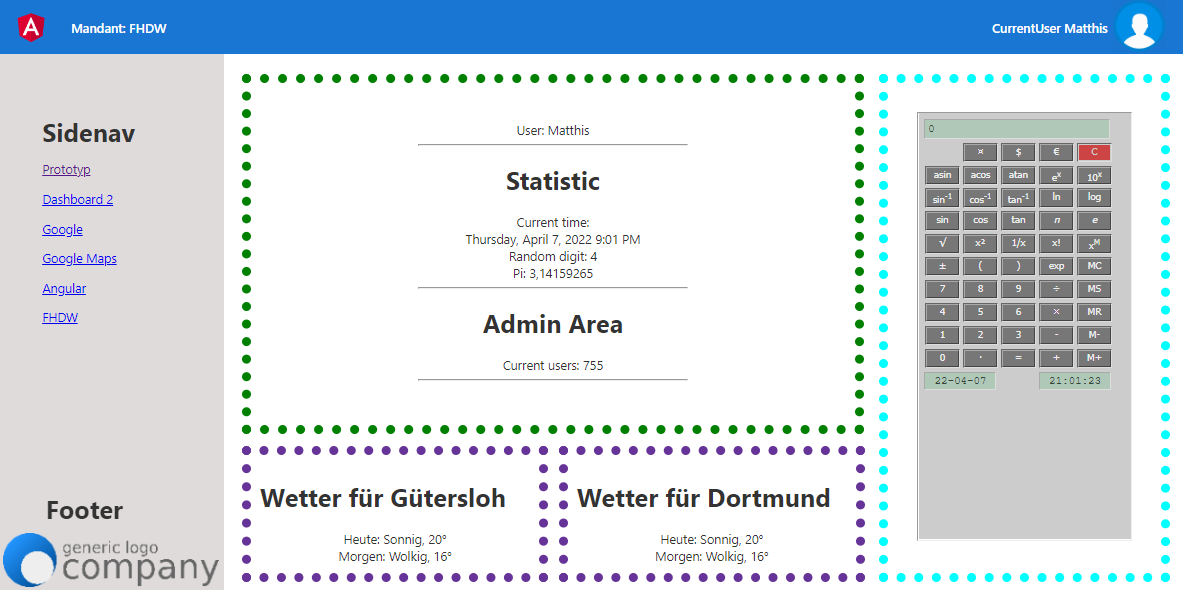
\includegraphics[width=1\textwidth]{img/PrototypMicrofrontends}}\\ % Pfad
		\source{Eigene Darstellung} % Quelle
		\label{fig:ImplementierungScreenshot}
	\end{minipage}
\end{figure}

Die implementierte Lösung gleicht dem Mockup aus \cref{fig:MockupBeispiel}, welche in \cref{sec:PrototypischesBeispiel} vorgestellt wurde. Die vier Microfrontendinstanzen sind nebeneinander dargestellt. Eine horizontale Trennung wurde ermöglicht, sodass mehrere Instanzen auf einer Seite dargestellt werden können. Die Microfrontends sind zur besseren Darstellung der Trennung mit einem farblichen Rahmen dargestellt.

Das Module Federation Microfrontend (grün) teilt einige seiner Bibliotheken mit der Portalshell. Zum jetzigen Zeitpunkt wird dadurch kaum Datenmenge eingespart. Aber wenn weitere Statistik-Apps eingebunden werden würden, würden diese von der Teilung der Bibliotheken profitieren. Die Statistik-App kann ihr Rechtekonzept anwenden. Sie bezieht die Informationen des angemeldeten Benutzers aus einer mit der Portalshell geteilten \texttt{AuthLib}\footnote{\cite[Sourcecode unter][]{Steyer2021f}}. Die \texttt{AuthLib} wird beim Login mit den Userdaten gefüllt und Module Federation Microfrontends können sie einbinden und Daten konsumieren.

Die geteilten Userinformationen (Benutzername: \textit{Matthis}) sind sowohl im Microfrontend, als auch im Header der Portalshell dargestellt und werden beide Male dynamisch aus der \texttt{AuthLib} bezogen. Da der User \textit{Matthis} die Rolle Admin zugeordnet hat, sieht er den erweiterten Admin-Bereich in der Statistik-App. Andere Komponenten können ebenfalls Daten aus der \texttt{AuthLib} konsumieren.

Die Wetter-App (lila) wurde doppelt mit unterschiedlichen Standorten als Web Component eingebunden. So konnte die Komponente nach einmaligem Einbinden wiederverwendet werden, ohne ein zweites Mal zum Client geladen zu werden.\footnote{Siehe \cref{fig:PrototypEinmaligesLadenWC} in Anhang \ref{app:Bilder}}

Das Taschenrechner Microfrontend (blau) konnte von \url{https://www.blitzrechner.de/taschenrechner-wissenschaftlich/} als Iframe eingebunden werden. Der benötigte Aufwand zum Einbinden der verschiedenen Arten skalierte mit den geschätzten Erkenntnissen des Aufwands von \cref{tab:MessungenEvaluierung} aus \cref{sec:EvaluierungIFrame} und war dementsprechend gering.

\textbf{Fazit}\\
Der in \cref{sec:Evaluierung} durch die Nutzwertanalyse entwickelte Entscheidungsbaum konnte an den Microfrontends des prototypischen Beispieles durchlaufen werden. Die Microfrontends wurden dadurch jeweils nach der geeignetsten Art in die Portalshell eingebunden. Durch die Erkenntnisse aus \cref{sec:ImplementierungValidierungKriterien} konnte bestätigt werden, dass der entwickelte Entscheidungsbaum anwendbar ist und sinnvolle Resultate erzielt.